\chapter{Attention Models}\label{ch:attention}

Attention mechanisms constitute the natural complement to the geometric convolutions developed in the previous chapter: where convolutions impose rigid structure through shared kernels with content-independent weights, attention introduces adaptive flexibility, dynamically weighting the contributions of each element according to the information it carries. This chapter develops the mathematical foundations of attention mechanisms, from their classical algebraic formulation to the geometric extensions that allow operating over non-Euclidean domains while preserving symmetries.

We start from traditional attention mechanisms, formalized as integral operators over Hilbert spaces, and then progressively incorporate geometric structure: first equivariance with respect to symmetry groups, then operation over graphs via attention networks and spectral analysis, the extension to Riemannian manifolds with parallel transport in hyperbolic and spherical spaces, the formulation in Clifford algebras that unifies scalars, vectors, and multivectors within a coherent algebraic framework, and finally attention over simplicial complexes and cohomological structures. Each extension incorporates richer geometric structure while preserving the dynamic adaptation capability that distinguishes attention from convolution.

This progression from the algebraic to the geometric connects directly with the preceding chapters: \autoref{ch:cnn} established that attention generalizes convolution as a limiting case when the Gaussian kernel relaxes its local support, and \autoref{ch:gdl} identified \glspl{Transformer} as instances of the \gls{MPNN} framework over adaptive complete graphs (\autoref{prop:attention_mpnn}). This chapter develops both connections in depth.

\section{Traditional Attention Mechanisms}\label{sec:atencion_tradicional}

\subsection{Introduction and History}\label{subsec:historia_atencion}

Attention mechanisms emerge historically from the need to overcome the inherent limitations of sequential models in natural language processing. The early works of \citet{bahdanau2014neural} and \citet{luong2015effective} introduced attention mechanisms in machine translation systems based on recurrent neural networks, allowing the model to ``attend'' to different parts of the input sequence during generation.

The turning point came with the seminal work \textit{"Attention is All You Need"} by \citet{vaswani2017attentionneed}, which demonstrated that attention mechanisms alone, without recurrence or convolution, could achieve state-of-the-art performance on machine translation tasks. This \gls{Transformer} architecture revolutionized not only natural language processing, but became the foundation of computer vision models, graph processing, and, eventually, geometric deep learning.

The historical evolution can be summarized in three main phases:

\begin{enumerate}
    \item \textbf{Attention as a complement} (2014-2016): Attention mechanisms added to \glspl{RNN} to improve the handling of long-range dependencies
    \item \textbf{Attention as the main architecture} (2017-2019): Pure \glspl{Transformer} replacing recurrent architectures
    \item \textbf{Geometric attention} (2020-present): Extension to non-Euclidean data with preservation of symmetries
\end{enumerate}

\subsection{Algebraic Foundations}\label{subsec:fundamentos_algebraicos_atencion}

Attention mechanisms are grounded in concepts from linear algebra and the geometry of vector spaces. At their core, attention operates over three interrelated vector spaces that encode different aspects of the information.

\subsubsection{Feature Spaces}\label{subsubsec:espacios_caracteristicas}

Consider a feature space $\mathcal{H} = \mathbb{R}^d$ where the input representations reside. For a set of $n$ input elements, we have:

\begin{equation}
    \mathbf{X} = [\mathbf{x}_1, \mathbf{x}_2, \ldots, \mathbf{x}_n]^T \in \mathbb{R}^{n \times d}
    \label{eq:input_matrix}
\end{equation}

where each $\mathbf{x}_i \in \mathcal{H}$ represents an element of the input sequence.

\subsubsection{Fundamental Linear Transformations}

The attention mechanism defines three fundamental linear transformations:

\begin{align}
    \mathbf{Q} &= \mathbf{X}\mathbf{W}_Q \in \mathbb{R}^{n \times d_k} \quad \text{(Queries)} \\
    \mathbf{K} &= \mathbf{X}\mathbf{W}_K \in \mathbb{R}^{n \times d_k} \quad \text{(Keys)} \\
    \mathbf{V} &= \mathbf{X}\mathbf{W}_V \in \mathbb{R}^{n \times d_v} \quad \text{(Values)}
    \label{eq:linear_projections}
\end{align}

where the weight matrices $\mathbf{W}_Q, \mathbf{W}_K \in \mathbb{R}^{d \times d_k}$ and $\mathbf{W}_V \in \mathbb{R}^{d \times d_v}$ are trainable parameters that project the input space into specialized subspaces.

The dimensions are related as follows: if $\mathbf{X} \in \mathbb{R}^{n \times d}$ represents $n$ elements with $d$ features each, then the projections result in queries and keys of dimension $d_k$ and values of dimension $d_v$. In the standard multi-head implementation, $d_k = d_v = d/h$ is used, where $h$ is the number of attention heads.

\begin{definition}[Dot Product as a Similarity Measure]\label{def:dot_product_similarity}
    The fundamental compatibility function in attention is defined via the dot product:
    \begin{equation}
        \text{sim}(\mathbf{q}_i, \mathbf{k}_j) = \mathbf{q}_i^T \mathbf{k}_j = \|\mathbf{q}_i\| \|\mathbf{k}_j\| \cos(\theta_{ij})
        \label{eq:dot_product_similarity}
    \end{equation}
    where $\theta_{ij}$ is the angle between the vectors $\mathbf{q}_i$ and $\mathbf{k}_j$.
\end{definition}

This geometric interpretation reveals that attention measures the normalized cosine similarity between representations in the feature space.

\subsubsection{Geometry of the Q, K, V Spaces}

The underlying geometric structure of the query, key, and value spaces provides deep insights into how attention works.

\begin{definition}[Similarity Matrix in the Attention Space]\label{def:gram_metric_attention}
    The \textit{similarity matrix} (or cross inner-product matrix) associated with the queries and keys is defined as:
    \begin{equation}
        \mathbf{S} = \mathbf{Q}\mathbf{K}^T, \quad S_{ik} = \langle \mathbf{q}_i, \mathbf{k}_k \rangle \in \mathbb{R}^{n \times n}
        \label{eq:gram_matrix_attention}
    \end{equation}
    This matrix encodes all the geometric relations between queries and keys. When $\mathbf{Q} = \mathbf{K}$ (pure self-attention), $\mathbf{S}$ coincides with the Gram matrix of the keys.
\end{definition}

\begin{proposition}[Geometric Properties of the Similarity Matrix]\label{prop:geometric_properties_gram}
    The matrix $\mathbf{S} = \mathbf{Q}\mathbf{K}^T$ satisfies:
    \begin{enumerate}
        \item \textbf{Singular value decomposition}: $\mathbf{S} = \mathbf{U}\mathbf{\Sigma}\mathbf{V}^T$ (SVD), where $\mathbf{U}, \mathbf{V}$ capture the principal directions of queries and keys respectively and $\mathbf{\Sigma}$ contains the singular values.
        \item \textbf{Frobenius norm}: $\|\mathbf{S}\|_F^2 = \text{tr}(\mathbf{Q}\mathbf{K}^T\mathbf{K}\mathbf{Q}^T) = \|\mathbf{K}\mathbf{Q}^T\|_F^2$
        \item \textbf{Angular interpretation}: $S_{ij} = \|\mathbf{q}_i\|\|\mathbf{k}_j\|\cos(\theta_{ij})$, where $\theta_{ij}$ is the angle between $\mathbf{q}_i$ and $\mathbf{k}_j$.
    \end{enumerate}
\end{proposition}

\begin{proof}
    Property (1) is the standard singular value decomposition, applicable to every real matrix. Property (2) follows from $\|\mathbf{S}\|_F^2 = \text{tr}(\mathbf{S}\mathbf{S}^T) = \text{tr}(\mathbf{Q}\mathbf{K}^T(\mathbf{Q}\mathbf{K}^T)^T) = \text{tr}(\mathbf{Q}\mathbf{K}^T\mathbf{K}\mathbf{Q}^T)$, and by the cyclic property of the trace, $\text{tr}(\mathbf{Q}\mathbf{K}^T\mathbf{K}\mathbf{Q}^T) = \text{tr}(\mathbf{K}\mathbf{Q}^T\mathbf{Q}\mathbf{K}^T) = \|\mathbf{K}\mathbf{Q}^T\|_F^2$. Property (3) is an immediate consequence of the definition of the inner product in Euclidean spaces.
\end{proof}

\begin{theorem}[Geometric Projection Theorem in Attention]\label{theorem:geometric_projection_attention}
    The attention mechanism can be interpreted as a geometric projection of the value space $\mathcal{V}$ onto the subspace generated by the queries $\text{span}(\mathbf{Q})$, mediated by the metric induced by the keys.

    Formally, for each query $\mathbf{q}_i$:
    \begin{equation}
        \mathbf{y}_i = \sum_{j=1}^n \alpha_{ij} \mathbf{v}_j = \mathbf{V}^T \boldsymbol{\alpha}_i
        \label{eq:geometric_projection_formula}
    \end{equation}
    where $\boldsymbol{\alpha}_i = \text{softmax}(\mathbf{G}_{i,:}/\sqrt{d_k})$ defines a probability distribution over the value index.
\end{theorem}

\begin{proof}
    The proof proceeds by recognizing that the attention weights $\alpha_{ij}$ form a convex (probabilistic) combination over the values. This combination is determined by the geometric proximity between $\mathbf{q}_i$ and each key $\mathbf{k}_j$, measured by the scaled inner product and normalized by softmax.

    The resulting projection preserves the structure of the value space while emphasizing directions aligned with the query according to the metric defined by the keys.
\end{proof}

\begin{figure}[ht]
    \centering
    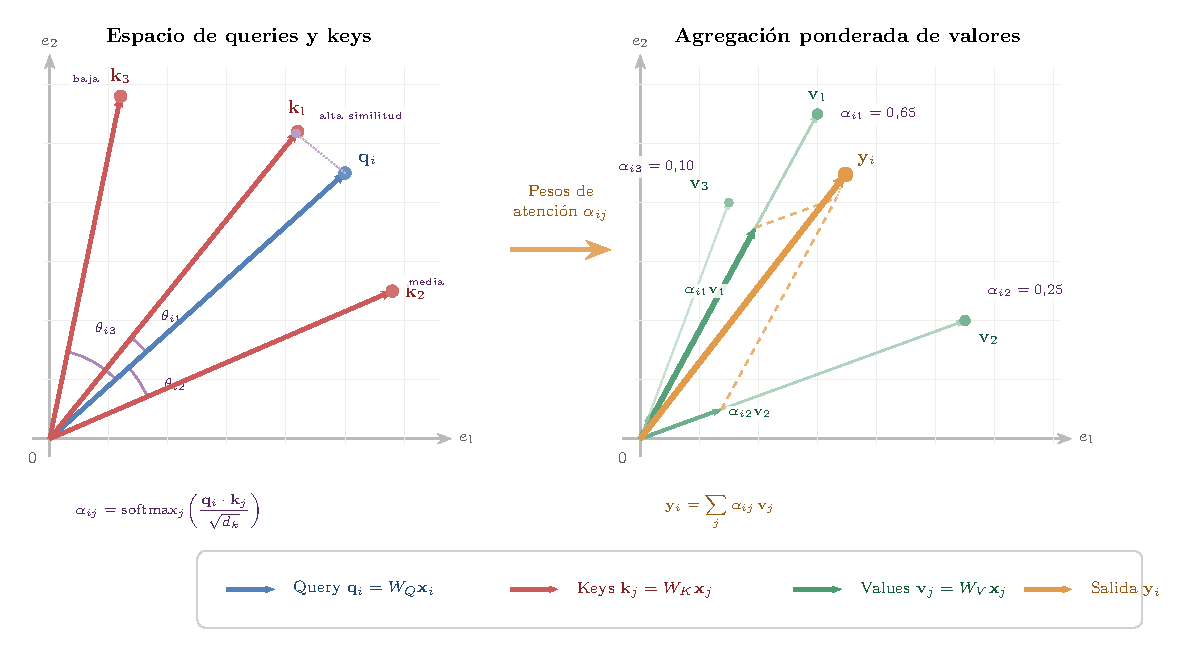
\includegraphics[width=0.95\textwidth]{images/qkv_geometric_projection.pdf}
    \caption{Geometric interpretation of the attention mechanism. \textbf{Left}: in the space of queries and keys, the similarity between $\mathbf{q}_i$ and each $\mathbf{k}_j$ is measured by the angle $\theta_{ij}$ (scaled inner product). \textbf{Right}: the values $\mathbf{v}_j$ are weighted by the attention weights $\alpha_{ij}$, and the output $\mathbf{y}_i$ is their convex combination.}
    \label{fig:qkv_geometric_projection}
\end{figure}

\subsubsection{Multiresolution Analysis of Attention}

The analysis of attention from a harmonic analysis perspective reveals hierarchical structure at multiple scales.

\begin{definition}[Attention Spectrum]\label{def:attention_spectrum}
    For an attention matrix $\mathbf{A} = \text{softmax}(\mathbf{Q}\mathbf{K}^T/\sqrt{d_k})$, we define its \textit{spectrum} as the set of eigenvalues:
    \begin{equation}
        \text{Spec}(\mathbf{A}) = \{\lambda_1, \lambda_2, \ldots, \lambda_n : \mathbf{A}\mathbf{v}_i = \lambda_i \mathbf{v}_i\}
        \label{eq:attention_spectrum}
    \end{equation}
    The eigenvectors $\{\mathbf{v}_i\}$ reveal the principal attention patterns.
\end{definition}

\begin{example}[Explicit Computation: $3 \times 3$ Attention]\label{ex:explicit_3x3_attention}
    Consider a concrete example with $n=3$ elements and $d_k=2$:

    \begin{equation}
        \mathbf{Q} = \begin{bmatrix} 1 & 0 \\ 0 & 1 \\ 1 & 1 \end{bmatrix}, \quad
        \mathbf{K} = \begin{bmatrix} 1 & 0 \\ 1 & 1 \\ 0 & 1 \end{bmatrix}, \quad
        \mathbf{V} = \begin{bmatrix} 2 & 0 \\ 0 & 2 \\ 1 & 1 \end{bmatrix}
    \end{equation}

    \textbf{Step 1: Compatibility matrix}
    \begin{equation}
        \mathbf{S} = \mathbf{Q}\mathbf{K}^T = \begin{bmatrix} 1 & 1 & 0 \\ 0 & 1 & 1 \\ 1 & 2 & 1 \end{bmatrix}
    \end{equation}

    \textbf{Step 2: Attention matrix (without scaling, for simplicity)}
    \begin{equation}
        \mathbf{A} = \text{softmax}(\mathbf{S}) \approx \begin{bmatrix} 0.42 & 0.42 & 0.16 \\ 0.16 & 0.42 & 0.42 \\ 0.21 & 0.58 & 0.21 \end{bmatrix}
    \end{equation}

    \textbf{Step 3: Attention output}
    \begin{equation}
        \mathbf{Y} = \mathbf{A}\mathbf{V} \approx \begin{bmatrix} 1.00 & 1.00 \\ 0.74 & 1.26 \\ 0.63 & 1.37 \end{bmatrix}
    \end{equation}

    This example illustrates how different query-key patterns produce different convex combinations of values.
\end{example}

\subsection{Basic Attention Mechanism}\label{subsec:atencion_basico}

\subsubsection{Fundamental Attention Equation}

The scaled dot-product attention mechanism is formally defined as:

\begin{equation}
    \text{Attention}(\mathbf{Q}, \mathbf{K}, \mathbf{V}) = \text{softmax}\left(\frac{\mathbf{Q}\mathbf{K}^T}{\sqrt{d_k}}\right)\mathbf{V}
    \label{eq:scaled_dot_product_attention}
\end{equation}

The attention score matrix $\mathbf{S} = \mathbf{Q}\mathbf{K}^T \in \mathbb{R}^{n \times n}$ encodes the compatibility between each query-key pair, while the scaling factor $\frac{1}{\sqrt{d_k}}$ prevents the dot-product values from growing excessively with the dimension.

\subsubsection{Geometric Interpretation}

The attention operation can be interpreted as a convex interpolation in the value space:

\begin{equation}
    \mathbf{y}_i = \sum_{j=1}^{n} \alpha_{ij} \mathbf{v}_j, \quad \sum_{j=1}^{n} \alpha_{ij} = 1, \quad \alpha_{ij} \geq 0
    \label{eq:convex_combination}
\end{equation}

where the attention weights $\alpha_{ij}$ form a probability distribution over the values.

\begin{definition}[Generalized Attention Function]\label{def:generalized_attention}
    A \textit{generalized attention function} is a function $f: \mathcal{X}^n \times \mathcal{Y}^n \times \mathcal{Z}^n \to \mathcal{W}^n$ where:
    \begin{align}
        f(\mathbf{Q}, \mathbf{K}, \mathbf{V}) &= \sum_{j=1}^{n} \alpha_{ij} \mathbf{v}_j \\
        \alpha_{ij} &= \frac{\exp(e_{ij})}{\sum_{k=1}^{n} \exp(e_{ik})} \\
        e_{ij} &= a(\mathbf{q}_i, \mathbf{k}_j)
    \end{align}
    where $a: \mathcal{X} \times \mathcal{Y} \to \mathbb{R}$ is a compatibility function.
\end{definition}

\subsubsection{Self-Attention and Global Dependencies}

Self-attention constitutes the special case where the queries, keys, and values come from the same input:

\begin{equation}
    \mathbf{Q} = \mathbf{K} = \mathbf{V} = \mathbf{X}
    \label{eq:self_attention_case}
\end{equation}

This formulation allows each element of the sequence to attend to all the other elements, capturing global dependencies in a single operation.

\begin{theorem}[Universality of Self-Attention]\label{theorem:self_attention_universality}
    Let $K \subseteq \mathbb{R}^{n \times d}$ be a compact set. For any continuous function
    $f: K \to \mathbb{R}^{n \times d}$ that is permutation-equivariant (i.e., $f(P\mathbf{X}) = Pf(\mathbf{X})$
    for any permutation matrix $P$), there exists a self-attention network that can approximate
    $f$ uniformly on $K$ with arbitrary precision.

    This result extends the universal approximation theorems for symmetric functions
    \citep{zaheer2017deepsets} to the context of attention mechanisms. Full universality requires the complete Transformer architecture (self-attention combined with feed-forward layers and residual connections), not solely isolated self-attention layers; see the rigorous proof in \citet{yun2020transformers}.
\end{theorem}

\begin{proof}
    The proof proceeds in three main steps:

    \textbf{Step 1: Characterization of permutation-equivariant functions.}
    Let $f: K \to \mathbb{R}^{n \times d}$ be a continuous, permutation-equivariant function, where $K \subseteq \mathbb{R}^{n \times d}$ is compact. By the representation theorem for symmetric functions \citep{zaheer2017deepsets}, any permutation-equivariant function can be expressed as:

    \begin{equation}
        f(\mathbf{X})_i = \phi\left(\mathbf{x}_i, \sum_{j=1}^n \rho(\mathbf{x}_j)\right)
        \label{eq:symmetric_representation}
    \end{equation}

    where $\phi: \mathbb{R}^d \times \mathbb{R}^d \to \mathbb{R}^d$ and $\rho: \mathbb{R}^d \to \mathbb{R}^d$ are appropriate continuous functions.

    \textbf{Step 2: Approximation via pairwise interactions.}
    By the universal approximation theorem for neural networks, for any $\epsilon > 0$, there exist functions $g_1, g_2, g_3: \mathbb{R}^d \to \mathbb{R}^{d'}$ and $h: \mathbb{R}^{d'} \to \mathbb{R}^d$ such that:

    \begin{equation}
        \left\|f(\mathbf{X})_i - \sum_{j=1}^n \text{softmax}(g_1(\mathbf{x}_i)^T g_2(\mathbf{x}_j)) \cdot h(g_3(\mathbf{x}_j))\right\| < \epsilon
        \label{eq:pairwise_approximation}
    \end{equation}

    uniformly for $\mathbf{X} \in K$.

    \textbf{Step 3: Exact implementation via self-attention.}
    We define the projection matrices as:
    \begin{align}
        \mathbf{W}_Q &= \begin{bmatrix} \mathbf{W}_{g_1} \\ \mathbf{0} \end{bmatrix} \in \mathbb{R}^{d \times d_k} \\
        \mathbf{W}_K &= \begin{bmatrix} \mathbf{W}_{g_2} \\ \mathbf{0} \end{bmatrix} \in \mathbb{R}^{d \times d_k} \\
        \mathbf{W}_V &= \begin{bmatrix} \mathbf{W}_{g_3} \\ \mathbf{0} \end{bmatrix} \in \mathbb{R}^{d \times d_v}
    \end{align}

    where $\mathbf{W}_{g_1}, \mathbf{W}_{g_2}, \mathbf{W}_{g_3}$ implement the functions $g_1, g_2, g_3$ respectively via linear layers.

    With this construction, the self-attention mechanism produces exactly:
    \begin{equation}
        \text{SelfAttention}(\mathbf{X})_i = \sum_{j=1}^n \text{softmax}\left(\frac{g_1(\mathbf{x}_i)^T g_2(\mathbf{x}_j)}{\sqrt{d_k}}\right) h(g_3(\mathbf{x}_j))
        \label{eq:self_attention_implementation}
    \end{equation}

    The scaling factor $\sqrt{d_k}$ can be absorbed into the functions $g_1$ and $g_2$ without loss of generality.

    By composition of universally approximable functions and the density of continuous functions on compact spaces, we conclude that self-attention networks can uniformly approximate any continuous permutation-equivariant function on compact sets.
\end{proof}

\subsection{Multi-Head Attention}

\subsubsection{Decomposition into Parallel Subspaces}

The Multi-Head Attention mechanism extends basic attention through parallel processing in multiple representation subspaces:

\begin{equation}
    \text{MultiHead}(\mathbf{Q}, \mathbf{K}, \mathbf{V}) = \text{Concat}(\text{head}_1, \ldots, \text{head}_h)\mathbf{W}_O
    \label{eq:multihead_attention}
\end{equation}

where each attention head is defined as:

\begin{equation}
    \text{head}_i = \text{Attention}(\mathbf{Q}\mathbf{W}_Q^i, \mathbf{K}\mathbf{W}_K^i, \mathbf{V}\mathbf{W}_V^i)
    \label{eq:attention_head}
\end{equation}

with projection matrices $\mathbf{W}_Q^i, \mathbf{W}_K^i \in \mathbb{R}^{d \times d_k}$, $\mathbf{W}_V^i \in \mathbb{R}^{d \times d_v}$ for $i = 1, \ldots, h$.

\subsubsection{Advantages of the Decomposition}

The multi-head architecture provides several fundamental benefits:

\begin{enumerate}
    \item \textbf{Specialization of representations}: Each head can specialize in capturing different types of relations
    \item \textbf{Increased capacity}: The model can simultaneously attend to multiple positions and subspaces
    \item \textbf{Robustness}: The partial redundancy among heads improves training stability
\end{enumerate}

\begin{figure}[ht]
\centering
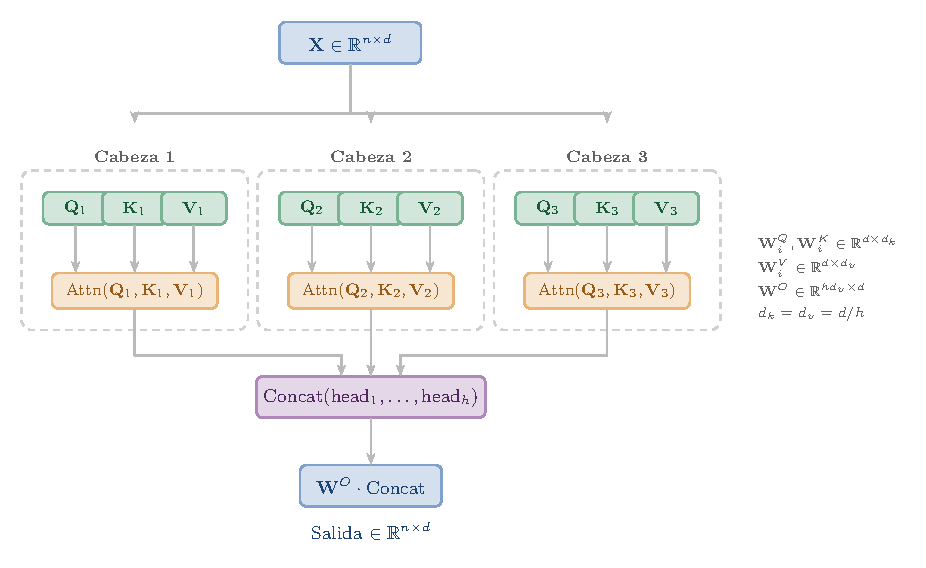
\includegraphics[width=0.85\textwidth]{images/multi_head_attention.pdf}
\caption{Diagram of Multi-Head Attention. The input is projected into $h$ parallel subspaces, each with its own matrices $\mathbf{W}^Q_i$, $\mathbf{W}^K_i$, $\mathbf{W}^V_i$. Each head computes attention independently, and the results are concatenated and projected via $\mathbf{W}^O$.}
\label{fig:multi_head_attention}
\end{figure}

\begin{proposition}[Multi-Head Representational Capacity for Pre-Softmax Scores]\label{theorem:multihead_representational_capacity}
    The Multi-Head Attention mechanism with $h$ heads can represent any pre-softmax score pattern that admits a decomposition as a sum of $h$ low-rank functions.

    Formally, if $\mathbf{S}^* = \sum_{i=1}^h \mathbf{U}_i \mathbf{\Sigma}_i \mathbf{V}_i^T$ where each $\mathbf{U}_i \mathbf{\Sigma}_i \mathbf{V}_i^T$ has rank $r_i \leq d_k$, then there exists a Multi-Head configuration with $h$ heads whose pre-softmax score matrix is exactly $\mathbf{S}^*$.
\end{proposition}

\begin{proof}
    The proof proceeds by direct construction. For each term $\mathbf{U}_i \mathbf{\Sigma}_i \mathbf{V}_i^T$ in the decomposition, we define the $i$-th head as:
    \begin{align}
        \mathbf{W}_Q^i &= \mathbf{U}_i \mathbf{\Sigma}_i^{1/2} \\
        \mathbf{W}_K^i &= \mathbf{V}_i \mathbf{\Sigma}_i^{1/2} \\
        \mathbf{W}_V^i &= \mathbf{I}
    \end{align}

    With this choice, the pre-softmax score matrix of head $i$ is $\mathbf{Q}_i \mathbf{K}_i^T = \mathbf{X}\mathbf{U}_i \mathbf{\Sigma}_i \mathbf{V}_i^T \mathbf{X}^T$, and the sum over heads reproduces the desired structure $\mathbf{S}^*$.
\end{proof}

\begin{remark}
The above construction operates at the level of pre-softmax scores. In practice, each head applies softmax to its scores before aggregation with the values, which introduces the constraint that the effective attention weights are non-negative and sum to 1 per row. This nonlinearity prevents the multi-head mechanism from exactly representing arbitrary attention functions at the output level.
\end{remark}

\subsubsection{Orthogonality Analysis Between Heads}

\begin{definition}[Functional Orthogonality Between Heads]\label{def:functional_orthogonality_heads}
    Two attention heads $\text{head}_i$ and $\text{head}_j$ are \textit{functionally orthogonal} if their projection matrices satisfy:
    \begin{equation}
        \langle \mathbf{W}_Q^i, \mathbf{W}_Q^j \rangle_F = \text{tr}((\mathbf{W}_Q^i)^T \mathbf{W}_Q^j) = 0
        \label{eq:head_orthogonality}
    \end{equation}
    where $\langle \cdot, \cdot \rangle_F$ denotes the Frobenius inner product.
\end{definition}

\begin{proposition}[Benefits of Orthogonality]\label{prop:orthogonality_benefits}
    If the attention heads are mutually orthogonal in the sense of \autoref{def:functional_orthogonality_heads}, then:
    \begin{enumerate}
        \item The information captured by each head is complementary (non-redundant)
        \item The Frobenius norm of the Multi-Head is the sum of the individual norms: $\|\text{MultiHead}\|_F^2 = \sum_{i=1}^h \|\text{head}_i\|_F^2$
        \item The gradient during backpropagation decomposes cleanly across heads
    \end{enumerate}
\end{proposition}

\begin{proof}
\leavevmode
\begin{enumerate}
    \item \textbf{Complementarity.} If $\langle \mathbf{W}_Q^i, \mathbf{W}_Q^j \rangle_F = 0$ for $i \neq j$, the query subspaces are orthogonal. Hence each head projects onto a distinct subspace of $\mathbb{R}^d$, capturing linearly independent information.

    \item \textbf{Norm decomposition.} The Multi-Head output is $\text{MultiHead} = \sum_{i=1}^h \text{head}_i \mathbf{W}_O^i$. By the orthogonality of the heads and Parseval's identity for orthogonal subspaces:
    \[
    \|\text{MultiHead}\|_F^2 = \left\|\sum_{i=1}^h \text{head}_i \mathbf{W}_O^i\right\|_F^2 = \sum_{i=1}^h \|\text{head}_i \mathbf{W}_O^i\|_F^2 = \sum_{i=1}^h \|\text{head}_i\|_F^2
    \]
    where the last equality assumes $\mathbf{W}_O^i$ orthonormal.

    \item \textbf{Gradients.} By orthogonality, $\frac{\partial \mathcal{L}}{\partial \mathbf{W}_Q^i}$ has no components in the direction of the subspaces of $\text{head}_j$ ($j \neq i$), avoiding interference between the updates of different heads. \qedhere
\end{enumerate}
\end{proof}

\subsubsection{Complexity Analysis}

The computational complexity of Multi-Head Attention is:

\begin{align}
    \text{Time} &: O(n^2 d + ndhd_k) \\
    \text{Space} &: O(n^2 + ndh)
\end{align}

where the $n^2$ term dominates for long sequences, motivating subsequent optimizations such as sparse and linear attention.

\subsection{Formalization as an Integral Operator}\label{subsec:attention_integral_operator}

The self-attention mechanism can be rigorously formalized as an integral operator acting on functions defined on manifolds, providing a deep mathematical perspective that connects with the classical theory of operators.

\subsubsection{Continuous Formulation}

Let $\mathcal{M}$ be a compact Riemannian manifold equipped with a measure $\mu$. For a function $f: \mathcal{M} \to \mathbb{R}^d$, the attention operator is defined as:

\begin{equation}
    \mathcal{T}f(x) = \int_{\mathcal{M}} K(x, y) f(y) \, d\mu(y)
    \label{eq:attention_integral_operator}
\end{equation}

where the \textbf{attention kernel} $K: \mathcal{M} \times \mathcal{M} \to \mathbb{R}^{d \times d}$ satisfies:

\begin{equation}
    K(x, y) = \sigma\left(\frac{\langle Q(x), K(y) \rangle}{\sqrt{d_k}}\right) V(y)^T
    \label{eq:attention_kernel}
\end{equation}

with $Q, K, V: \mathcal{M} \to \mathbb{R}^{d_k}, \mathbb{R}^{d_k}, \mathbb{R}^{d_v}$ respectively, and $\sigma$ the generalized softmax function.

\subsubsection{Properties of the Operator}

\begin{proposition}[Compactness of the Attention Operator]\label{prop:attention_compactness}
    If the kernel $K(x,y)$ is continuous on $\mathcal{M} \times \mathcal{M}$ and $\mathcal{M}$ is compact, then the operator $\mathcal{T}: L^2(\mathcal{M}) \to L^2(\mathcal{M})$ is compact.
\end{proposition}

\begin{proof}
    We will show that $\mathcal{T}: L^2(\mathcal{M}) \to L^2(\mathcal{M})$ is compact by applying the Arzelà-Ascoli criterion. To this end, we will show that the image of the unit ball $B = \{f \in L^2(\mathcal{M}) : \|f\|_{L^2} \leq 1\}$ under $\mathcal{T}$ is relatively compact in $C(\mathcal{M})$ (and therefore in $L^2(\mathcal{M})$).

    \textbf{Step 1: Uniform boundedness.}
    For $f \in B$ and $x \in \mathcal{M}$, we have:
    \begin{align}
        \|\mathcal{T}f(x)\| &= \left\|\int_{\mathcal{M}} K(x, y) f(y) \, d\mu(y)\right\| \\
        &\leq \int_{\mathcal{M}} \|K(x, y)\| \|f(y)\| \, d\mu(y) \\
        &\leq \sup_{x,y \in \mathcal{M}} \|K(x, y)\| \cdot \|f\|_{L^2} \cdot \sqrt{\mu(\mathcal{M})}
    \end{align}

    Since $K$ is continuous on the compact set $\mathcal{M} \times \mathcal{M}$, the function $\|K(x,y)\|$ attains its maximum. Therefore, $\{\mathcal{T}f : f \in B\}$ is uniformly bounded.

    \textbf{Step 2: Equicontinuity.}
    Let $x_1, x_2 \in \mathcal{M}$ and $f \in B$. Then:
    \begin{align}
        \|\mathcal{T}f(x_1) - \mathcal{T}f(x_2)\| &= \left\|\int_{\mathcal{M}} [K(x_1, y) - K(x_2, y)] f(y) \, d\mu(y)\right\| \\
        &\leq \int_{\mathcal{M}} \|K(x_1, y) - K(x_2, y)\| \|f(y)\| \, d\mu(y) \\
        &\leq \|f\|_{L^2} \sqrt{\mu(\mathcal{M})} \sup_{y \in \mathcal{M}} \|K(x_1, y) - K(x_2, y)\|
    \end{align}

    Since $K$ is continuous on the compact $\mathcal{M} \times \mathcal{M}$, it is uniformly continuous. Therefore, for any $\epsilon > 0$, there exists $\delta > 0$ such that if $d_{\mathcal{M}}(x_1, x_2) < \delta$, then:
    \[\sup_{y \in \mathcal{M}} \|K(x_1, y) - K(x_2, y)\| < \frac{\epsilon}{\sqrt{\mu(\mathcal{M})}}\]

    This implies $\|\mathcal{T}f(x_1) - \mathcal{T}f(x_2)\| < \epsilon$ for $f \in B$, establishing equicontinuity.

    \textbf{Step 3: Application of the Arzelà-Ascoli theorem.}
    By the previous steps, $\{\mathcal{T}f : f \in B\}$ is an equicontinuous and uniformly bounded family in $C(\mathcal{M})$. Since $\mathcal{M}$ is compact, the Arzelà-Ascoli theorem guarantees that this family is relatively compact in $C(\mathcal{M})$.

    Since $C(\mathcal{M})$ embeds densely in $L^2(\mathcal{M})$ and uniform convergence implies convergence in $L^2$, we conclude that $\mathcal{T}$ is a compact operator.
\end{proof}

\subsubsection{Connection with Spectral Analysis}

The integral formulation allows analyzing attention through spectral theory, following the analytical framework developed by \citet{sander2023attention}. The \textbf{eigenfunctions} of the operator $\mathcal{T}$ capture the fundamental attention patterns:

\begin{equation}
    \mathcal{T}\phi_i = \lambda_i \phi_i, \quad \lambda_1 \geq \lambda_2 \geq \cdots \geq 0
    \label{eq:attention_eigendecomposition}
\end{equation}

The eigenvalues $\lambda_i$ indicate the relative importance of each attention pattern, while the eigenfunctions $\phi_i$ define the principal directions in the feature space.

\begin{figure}[ht]
    \centering
    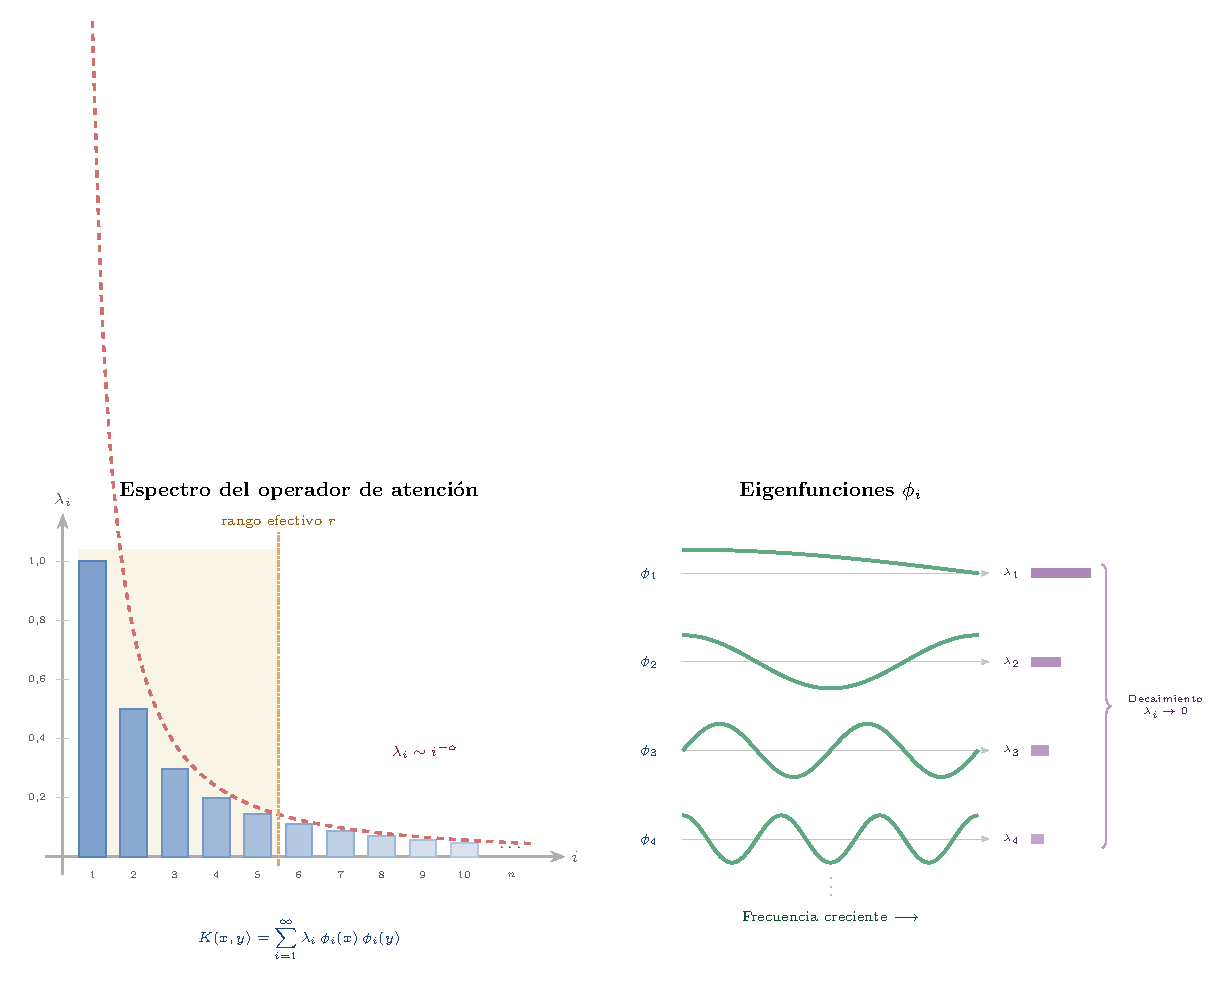
\includegraphics[width=0.95\textwidth]{images/attention_spectrum.pdf}
    \caption{Spectral decomposition of the attention operator. \textbf{Left}: the eigenvalues $\lambda_i$ of the attention kernel exhibit rapid decay ($\lambda_i \sim i^{-\alpha}$), which indicates a finite effective rank $r$ of the operator. The shaded region corresponds to the dominant modes. \textbf{Right}: the associated eigenfunctions $\phi_i$ show increasing frequency, analogously to the Fourier basis; the purple bars indicate the magnitude of the corresponding eigenvalue.}
    \label{fig:attention_spectrum}
\end{figure}

\subsubsection{Mercer Kernels and Advanced Spectral Theory}

The attention mechanism $\text{softmax}(QK^T/\sqrt{d})V$ can be interpreted as an integral operator with a data-dependent kernel. When this kernel satisfies the Mercer conditions (symmetry and positive definiteness), the powerful machinery of functional analysis (in particular the spectral theorem for compact operators) provides guarantees on the properties of the attention operator, such as its convergence and approximation capability.

\begin{definition}[Gaussian Attention Kernel]\label{def:gaussian_attention_kernel}
    A common variant of the attention kernel is the \textit{Gaussian kernel}:
    \begin{equation}
        K_{\text{gauss}}(x, y) = \exp\left(-\frac{\|Q(x) - K(y)\|^2}{2\sigma^2}\right)
        \label{eq:gaussian_attention_kernel}
    \end{equation}
    where $\sigma > 0$ is a scale parameter that controls the locality of the attention.
\end{definition}

\begin{theorem}[Spectral Decomposition of the Attention Kernel]\label{theorem:spectral_decomposition_attention}
    For an attention kernel $K: \mathcal{X} \times \mathcal{X} \to \mathbb{R}$ that is a Mercer kernel, there exists a spectral decomposition:
    \begin{equation}
        K(x, y) = \sum_{i=1}^{\infty} \lambda_i \phi_i(x) \phi_i(y)
        \label{eq:mercer_decomposition_attention}
    \end{equation}
    where $\{\lambda_i\}$ are non-negative eigenvalues in decreasing order and $\{\phi_i\}$ are orthonormal eigenfunctions.

    The corresponding attention operator admits the representation:
    \begin{equation}
        \mathcal{T}f = \sum_{i=1}^{\infty} \lambda_i \langle f, \phi_i \rangle_{L^2} \phi_i
        \label{eq:spectral_representation_attention}
    \end{equation}
\end{theorem}

\begin{proof}
    The proof follows from the spectral theorem for compact self-adjoint operators. Since $K$ is a Mercer kernel, the associated integral operator $\mathcal{T}$ is compact and positive. The spectral theorem guarantees the existence of the spectral decomposition, where the eigenvalues are real and non-negative.

    The convergence of the series is in the $L^2$ norm, and the spectral representation provides a complete characterization of the behavior of the operator.
\end{proof}

\begin{corollary}[Automatic Spectral Filtering]\label{cor:spectral_filtering}
    The attention operator acts as a natural low-pass filter, where:
    \begin{enumerate}
        \item High-frequency components (small eigenvalues) are attenuated
        \item The eigenvalue decay rate determines the smoothness of the attention function
        \item The effective rank of the operator is determined by the number of significant eigenvalues
    \end{enumerate}
\end{corollary}

\begin{proof}
Direct consequence of \autoref{theorem:spectral_decomposition_attention}. By the spectral representation $\mathcal{T}f = \sum_{i=1}^\infty \lambda_i \langle f, \phi_i \rangle \phi_i$ with eigenvalues in decreasing order $\lambda_1 \geq \lambda_2 \geq \cdots \geq 0$: (1)~the high-frequency components (large index $i$) are multiplied by small eigenvalues $\lambda_i$, attenuating them naturally; (2)~the decay rate $\lambda_i \to 0$ controls the smoothness of $\mathcal{T}f$ (rapid decay implies greater regularity); (3)~the effective rank is $r_\epsilon = |\{i : \lambda_i > \epsilon\}|$, which determines the intrinsic dimensionality of the representation.
\end{proof}

\subsubsection{Spectral Convergence Analysis}

\begin{theorem}[Convergence of Finite-Rank Approximations]\label{theorem:finite_rank_convergence}
    Let $\mathcal{T}_r$ be the rank-$r$ approximation of the attention operator:
    \begin{equation}
        \mathcal{T}_r f = \sum_{i=1}^{r} \lambda_i \langle f, \phi_i \rangle \phi_i
        \label{eq:finite_rank_approximation}
    \end{equation}

    Then, for any $f \in L^2(\mathcal{M})$:
    \begin{equation}
        \|\mathcal{T}f - \mathcal{T}_r f\|_{L^2} \leq \lambda_{r+1} \|f\|_{L^2}
        \label{eq:approximation_error_bound}
    \end{equation}
\end{theorem}

\begin{proof}
    By the spectral representation:
    \begin{align}
        \mathcal{T}f - \mathcal{T}_r f &= \sum_{i=r+1}^{\infty} \lambda_i \langle f, \phi_i \rangle \phi_i \\
        \|\mathcal{T}f - \mathcal{T}_r f\|_{L^2}^2 &= \sum_{i=r+1}^{\infty} \lambda_i^2 |\langle f, \phi_i \rangle|^2 \\
        &\leq \lambda_{r+1}^2 \sum_{i=r+1}^{\infty} |\langle f, \phi_i \rangle|^2 \\
        &\leq \lambda_{r+1}^2 \|f\|_{L^2}^2
    \end{align}
    where the last inequality uses Parseval's identity.
\end{proof}

\subsubsection{Physical and Geometric Interpretation}

The spectral analysis reveals that attention mechanisms naturally implement principles of harmonic analysis:

\begin{enumerate}
    \item \textbf{Decomposition into modes}: The eigenfunctions $\phi_i$ represent fundamental "attention modes"
    \item \textbf{Hierarchy of importance}: The eigenvalues $\lambda_i$ order these modes by importance
    \item \textbf{Implicit regularization}: The decay of eigenvalues provides automatic regularization
    \item \textbf{Frequency interpretation}: Modes with large eigenvalues correspond to "low-frequency" patterns in the feature space
\end{enumerate}

\textbf{Connection with Fourier Analysis.}\label{rem:fourier_connection} When the attention kernel is translation-invariant, the spectral decomposition reduces to classical Fourier analysis, where the eigenfunctions are complex exponentials and the eigenvalues are related to the Fourier transform of the kernel.

\subsubsection{Computational Applications}

The spectral analysis has important practical implications:

\begin{itemize}
    \item \textbf{Model compression}: Truncating the spectral expansion reduces the computational cost
    \item \textbf{Capacity analysis}: The effective rank indicates the representational capacity
    \item \textbf{Initialization}: The spectral modes can guide the initialization of weights
    \item \textbf{Regularization}: Penalizing large eigenvalues prevents overfitting
\end{itemize}

\begin{theorem}[Approximation by Finite Attention]\label{theorem:finite_attention_approximation}
    Let $\{x_i\}_{i=1}^n$ be an $\epsilon$-dense discretization of $\mathcal{M}$. The discrete attention operator:
    \begin{equation}
        \mathcal{T}_n f(x_i) = \sum_{j=1}^n \alpha_{ij} f(x_j), \quad \alpha_{ij} = \frac{\exp(K(x_i, x_j))}{\sum_{k=1}^n \exp(K(x_i, x_k))}
    \end{equation}
    converges to the continuous operator $\mathcal{T}$ in operator norm as $n \to \infty$ and $\epsilon \to 0$.
\end{theorem}

\begin{proof}[Sketch]
Let $f \in L^2(\mathcal{M})$ and $\mathcal{T}f(x) = \int_{\mathcal{M}} \alpha(x,y) f(y) \, d\mu(y)$ the continuous operator. The discrete approximation is $\mathcal{T}_n f(x_i) = \sum_{j=1}^n \alpha_{ij} f(x_j)$, which can be seen as a quadrature rule. For an $\epsilon$-dense discretization, the density of the points ensures that $|\mu(B_\epsilon(x_i)) - 1/n| \to 0$. The error decomposes into: (1) quadrature error $\|\mathcal{T}f - \mathcal{T}_n f\| = O(\epsilon^s)$ for $C^s$ kernels, by convergence of Riemann sums over compact manifolds; and (2) normalization error $|\sum_k \exp(K(x_i,x_k)) - \int \exp(K(x_i,y)) d\mu(y)| \to 0$ by the same argument. Under kernel regularity conditions (Lipschitz in both arguments), both errors converge to zero uniformly.
\end{proof}

This formulation reveals that standard \glspl{Transformer} can be seen as discrete approximations of integral operators over manifolds, providing a solid theoretical basis for geometric extensions.

\subsection{Functional Analysis of Attention}\label{subsec:functional_analysis_attention}

The theory of reproducing kernel Hilbert spaces (RKHS) provides a rigorous framework for understanding the functional properties of attention mechanisms.

\subsubsection{Attention as an Operator in RKHS}

\begin{definition}[Attention Kernel as a Mercer Kernel]\label{def:attention_mercer_kernel}
    The attention kernel $K_{\text{att}}: \mathcal{X} \times \mathcal{X} \to \mathbb{R}$ defined by:
    \begin{equation}
        K_{\text{att}}(x, y) = \exp\left(\frac{\langle Q(x), K(y) \rangle}{\sqrt{d_k}}\right)
        \label{eq:attention_mercer_kernel}
    \end{equation}
    is a \textit{Mercer kernel} if it is symmetric and positive definite.
\end{definition}

\begin{theorem}[RKHS Induced by Attention]\label{theorem:attention_rkhs}
    If $K_{\text{att}}$ is a Mercer kernel, then there exists a Hilbert space $\mathcal{H}_{\text{att}}$ with reproducing kernel such that:
    \begin{enumerate}
        \item $K_{\text{att}}(x, \cdot) \in \mathcal{H}_{\text{att}}$ for all $x \in \mathcal{X}$
        \item $\langle f, K_{\text{att}}(x, \cdot) \rangle_{\mathcal{H}_{\text{att}}} = f(x)$ for all $f \in \mathcal{H}_{\text{att}}$ (reproducing property)
        \item Attention can be expressed as: $\text{Attention}(x) = \sum_{i} \alpha_i K_{\text{att}}(x, x_i) V_i$
    \end{enumerate}
\end{theorem}

\begin{proof}
    The proof follows the standard Moore-Aronszajn construction:

    \textbf{Step 1}: We define the pre-Hilbert $\mathcal{H}_0$ as the linear span of $\{K_{\text{att}}(x, \cdot) : x \in \mathcal{X}\}$.

    \textbf{Step 2}: The inner product is defined by bilinearity:
    \[\left\langle \sum_i \alpha_i K_{\text{att}}(x_i, \cdot), \sum_j \beta_j K_{\text{att}}(y_j, \cdot) \right\rangle = \sum_{i,j} \alpha_i \beta_j K_{\text{att}}(x_i, y_j)\]

    \textbf{Step 3}: $\mathcal{H}_{\text{att}}$ is the completion of $\mathcal{H}_0$ under this norm.

    The reproducing property is verified directly by construction.
\end{proof}

\subsubsection{Regularization and Stability}

\begin{proposition}[Lipschitz Stability for Attention]\label{prop:lipschitz_stability_attention}
    If the functions $Q, K, V$ are $L$-Lipschitz and the data satisfy $\|x\|, \|y\| \leq R$ (essential boundedness hypothesis, since standard self-attention is not Lipschitz on unbounded domains), then the attention operator satisfies:
    \begin{equation}
        \|\text{Attention}(x) - \text{Attention}(y)\| \leq C_L \|x - y\|
        \label{eq:lipschitz_bound_attention}
    \end{equation}
    where $C_L$ depends on $L$, $R$, $d_k$ and the number of input elements $n$.
\end{proposition}

\begin{proof}
Let $\alpha_j(x) = \frac{\exp(\langle Q(x), K(x_j)\rangle / \sqrt{d_k})}{\sum_l \exp(\langle Q(x), K(x_l)\rangle / \sqrt{d_k})}$ be the attention weights. The softmax function is Lipschitz with constant 1 in the $\ell^\infty$ norm. Since $Q$ and $K$ are $L$-Lipschitz and $\|x\| \leq R$, the function $x \mapsto \langle Q(x), K(x_j)\rangle / \sqrt{d_k}$ is Lipschitz with constant $O(LR/\sqrt{d_k})$. Composing with softmax and the linear combination with $V(x_j)$ (also $L$-Lipschitz and bounded), one obtains $\|\text{Attention}(x) - \text{Attention}(y)\| \leq C_L \|x - y\|$ where $C_L = O(nL^2R/\sqrt{d_k})$. For a detailed derivation, see \citep{kim2021lipschitz}.
\end{proof}

\begin{theorem}[Automatic Spectral Regularization]\label{theorem:spectral_regularization}
    The attention operator acts as a natural spectral regularizer, filtering high-frequency components according to:
    \begin{equation}
        \|\mathcal{T}f\|_{\dot{H}^s} \leq C_s \|f\|_{\dot{H}^{s-\sigma}}
        \label{eq:spectral_regularization}
    \end{equation}
    where $\dot{H}^s$ denotes the homogeneous Sobolev space and $\sigma > 0$ is the order of regularization determined by the smoothness of the attention kernel.
\end{theorem}

\begin{proof}
By the spectral representation (\autoref{theorem:spectral_decomposition_attention}), $\mathcal{T}f = \sum_i \lambda_i \langle f, \phi_i\rangle \phi_i$. In the Sobolev norm $\dot{H}^s$, the $i$-th component has weight $\mu_i^s$ where $\mu_i$ are the eigenvalues of the Laplacian of $\mathcal{M}$. Then:
\[
\|\mathcal{T}f\|_{\dot{H}^s}^2 = \sum_i \lambda_i^2 \mu_i^{2s} |\langle f, \phi_i\rangle|^2
\]
If the attention kernel $K$ has Sobolev regularity $\sigma$ (that is, $\lambda_i = O(\mu_i^{-\sigma})$ as $i \to \infty$), then $\lambda_i^2 \mu_i^{2s} \leq C_s^2 \mu_i^{2(s-\sigma)}$, from which $\|\mathcal{T}f\|_{\dot{H}^s} \leq C_s \|f\|_{\dot{H}^{s-\sigma}}$.
\end{proof}

\begin{remark}
The above proof implicitly assumes that the eigenfunctions $\phi_i$ of the attention operator coincide (or are closely related) with the eigenfunctions of the Laplacian of $\mathcal{M}$. This assumption holds for isotropic kernels that commute with the Laplacian (for example, Matérn kernels on compact manifolds), but it is not valid for general attention kernels.
\end{remark}

\subsubsection{Convergence and Approximation}

\begin{theorem}[Monte Carlo Convergence for Attention]\label{theorem:monte_carlo_convergence}
    Let $\mathcal{T}_n$ be the discrete attention operator with $n$ points sampled i.i.d. according to a measure $\mu$. Then:
    \begin{equation}
        \mathbb{E}[\|\mathcal{T}_n - \mathcal{T}\|_{L^2 \to L^2}^2] \leq \frac{C}{n}
        \label{eq:monte_carlo_rate}
    \end{equation}
    where $C$ is a constant that depends on the properties of the kernel and the measure.
\end{theorem}

\begin{proof}
We consider the version with $1/n$ normalization (without softmax) to facilitate the analysis. The continuous operator is $\mathcal{T}f(x) = \int_\mathcal{M} K(x,y) f(y)\, d\mu(y)$ and its Monte Carlo approximation is $\mathcal{T}_n f(x) = \frac{1}{n}\sum_{j=1}^n K(x, y_j) f(y_j)$ with $y_j \sim \mu$ i.i.d. For fixed $f$, $\mathcal{T}_n f(x)$ is the empirical mean of $n$ i.i.d. random variables $Z_j = K(x, y_j)f(y_j)$ with expectation $\mathcal{T}f(x)$. For the rate:
\[
\mathbb{E}[\|\mathcal{T}_n f - \mathcal{T}f\|_{L^2}^2] = \frac{1}{n}\int_\mathcal{M} \text{Var}(K(x,\cdot)f(\cdot))\, d\mu(x) \leq \frac{C}{n}
\]
where $C = \|K\|_\infty^2 \|f\|_{L^2}^2 \mu(\mathcal{M})$. The extension to operator norm and to the case with softmax normalization (as in the statement) requires additional covering arguments and control of the convergence of the denominator, respectively.
\end{proof}

\section{Group Theory and Equivariance}

The incorporation of geometric symmetries into attention mechanisms constitutes one of the most significant developments in geometric deep learning, allowing models to preserve fundamental structures of the data.

\subsection{Foundations of Group Theory}

The foundations of group theory (groups, group actions, equivariance) needed for equivariant attention mechanisms are developed in full in \autoref{ch:gdl}, Sections~\ref{subsec:teoria_grupos_representaciones} and~\ref{subsec:equivarianza_invarianza}.

Attention mechanisms extend these principles through adaptive operations that preserve the symmetries of arbitrary groups, overcoming the fixed-equivariance limitations of \glspl{CNN}.

\subsubsection{Relevant Groups for Geometric Attention}

In the context of attention mechanisms, the most important groups include:

\begin{enumerate}
    \item \textbf{$SO(3)$}: 3D rotations, essential for Point \glspl{Transformer} and molecular data
    \item \textbf{$SE(3)$}: Special Euclidean group, fundamental in SE(3)-\glspl{Transformer}
    \item \textbf{$E(3)$}: Full Euclidean group, including reflections
    \item \textbf{General Lie groups}: Unified framework for Lie\glspl{Transformer}
    \item \textbf{Permutation groups}: For invariance to reorderings in sets
\end{enumerate}

\autoref{theorem:equivariant_composition} of \autoref{ch:gdl} ensures that equivariant attention layers can be composed while preserving the desired symmetry properties.

\subsection{Equivariant Attention}\label{subsec:equivariant_attention}\label{sec:equivariant_attention}

\subsubsection{Definition and Construction}

Applying the definition of equivariance from \autoref{ch:gdl} (\autoref{def:equivariance_gdl}) to attention mechanisms, an attention model is $G$-equivariant if it preserves the group transformations in queries, keys, and values.

\begin{theorem}[Construction of Equivariant Attention]
    For a group $G$ acting on the feature space, an attention mechanism is $G$-equivariant if and only if:
    \begin{enumerate}
        \item The compatibility functions are $G$-invariant
        \item The query, key, and value transformations commute with the group action
    \end{enumerate}
\end{theorem}

\begin{proof}[Proof sketch]
\textbf{Forward direction} ($\Leftarrow$): If the compatibility functions $a(\mathbf{q}_i, \mathbf{k}_j)$ are $G$-invariant, then $a(\rho(g)\mathbf{q}_i, \rho(g)\mathbf{k}_j) = a(\mathbf{q}_i, \mathbf{k}_j)$ for all $g \in G$, so the attention weights $\alpha_{ij}$ are invariant. If, moreover, the value transformations commute with $G$ ($W_V \rho(g) = \rho(g) W_V$), the output $\sum_j \alpha_{ij} W_V \rho(g)\mathbf{x}_j = \rho(g) \sum_j \alpha_{ij} W_V \mathbf{x}_j$, which gives equivariance.

\textbf{Converse direction} ($\Rightarrow$): If the attention is $G$-equivariant, the weights $\alpha_{ij}$ must be invariant under the simultaneous action of $G$ on Q and K (since they determine the linear combination), which requires invariance of the compatibility functions. The equivariance of the output with fixed weights implies that $W_V$ commutes with $\rho(g)$.
\end{proof}

\begin{lemma}[Sufficient Condition for Equivariance in Self-Attention]\label{lemma:self_attention_equivariance}
Let $G$ be a group acting on the input space $\mathbb{R}^{n \times d}$ via permutations.
If the projection matrices satisfy $\mathbf{W}_Q = \mathbf{W}_K = \mathbf{W}_V = \mathbf{W}$
and $\mathbf{W}$ commutes with the group action, then the self-attention mechanism
is $G$-equivariant.
\end{lemma}

\begin{proof}
For any permutation $P \in G$ and input $\mathbf{X} \in \mathbb{R}^{n \times d}$, we have:
\begin{align}
\text{SelfAttention}(P\mathbf{X}) &= \text{softmax}\left(\frac{(P\mathbf{X}\mathbf{W})(P\mathbf{X}\mathbf{W})^T}{\sqrt{d_k}}\right)(P\mathbf{X}\mathbf{W}) \\
&= \text{softmax}\left(\frac{P(\mathbf{X}\mathbf{W})(\mathbf{X}\mathbf{W})^T P^T}{\sqrt{d_k}}\right)P(\mathbf{X}\mathbf{W}) \\
&= P \cdot \text{SelfAttention}(\mathbf{X})
\end{align}
where the second step uses commutativity and the third the equivariance of softmax to permutations.
\end{proof}

\subsubsection{Irreducible Representations}

The theory of irreducible representations (\autoref{def:representacion_irreducible}, \autoref{ch:gdl}) provides the fundamental mathematical framework for designing equivariant attention mechanisms under compact Lie groups. This theory, developed initially by \citet{Peter1927} and extended to the context of deep learning by \citet{kondor2018generalizationconvolutionalneural}, establishes that any representation of a compact group decomposes into fundamental irreducible blocks.

By the Peter-Weyl theorem (\autoref{thm:peter_weyl}, \autoref{ch:gdl}), every representation decomposes into a direct sum of irreducible representations:
\begin{equation}
V = \bigoplus_{\lambda \in \widehat{G}} n_\lambda \mathcal{H}_\lambda
\label{eq:peter_weyl_decomposition_attention}
\end{equation}
where $\widehat{G}$ indexes the inequivalent irreducible representations, $\mathcal{H}_\lambda$ are the representation spaces, and $n_\lambda$ are the multiplicities.

\paragraph{Irreducible Representations of SO(3)}

For the group of three-dimensional rotations $SO(3)$, the irreducible representations are classified by a non-negative integer $\ell \in \mathbb{N}_0$ called the \textit{degree} or \textit{angular momentum}. Each irreducible representation has dimension $2\ell + 1$.

\begin{theorem}[Classification of Irreps of SO(3)]\label{thm:so3_irreps}
The irreducible representations of $SO(3)$ are indexed by $\ell \in \mathbb{N}_0$ and have dimension $d_\ell = 2\ell + 1$. The representation space $\mathcal{H}_\ell$ is generated by the spherical harmonics $Y_\ell^m$ with $m \in \{-\ell, -\ell+1, \ldots, \ell-1, \ell\}$.
\end{theorem}

\begin{proof}[Sketch]
The classification is established through the relation between $SO(3)$ and $SU(2)$. The Lie algebra $\mathfrak{so}(3) \cong \mathfrak{su}(2)$ has generators $\{J_x, J_y, J_z\}$ with commutation relations $[J_i, J_j] = i\epsilon_{ijk}J_k$. The Casimir operator $\mathbf{J}^2 = J_x^2 + J_y^2 + J_z^2$ commutes with the entire algebra, and by Schur's lemma it acts as a scalar on each irreducible. The simultaneous diagonalization of $\mathbf{J}^2$ and $J_z$ produces eigenvalues $\ell(\ell+1)$ and $m$ respectively, with $-\ell \leq m \leq \ell$, giving dimension $2\ell+1$. The spherical harmonics $Y_\ell^m$ realize these representations as functions on $S^2$. See \citep{brocker1985representations} for a complete proof.
\end{proof}

\begin{definition}[Spherical Harmonics]\label{def:spherical_harmonics_attention}
The \textit{spherical harmonics} $Y_\ell^m: S^2 \to \mathbb{C}$ of degree $\ell$ and order $m$ are eigenfunctions of the Laplacian operator on the sphere:
\begin{equation}
Y_\ell^m(\theta, \phi) = \sqrt{\frac{2\ell+1}{4\pi}\frac{(\ell-m)!}{(\ell+m)!}} P_\ell^m(\cos\theta) e^{im\phi}
\label{eq:spherical_harmonics_definition}
\end{equation}
where $P_\ell^m$ are the associated Legendre polynomials. Under a rotation $R \in SO(3)$, the spherical harmonics transform according to:
\begin{equation}
(R \cdot Y_\ell^m)(\mathbf{x}) = Y_\ell^m(R^{-1}\mathbf{x}) = \sum_{m'=-\ell}^{\ell} D_\ell^{m'm}(R) Y_\ell^{m'}(\mathbf{x})
\label{eq:spherical_harmonics_transformation}
\end{equation}
where $D_\ell^{m'm}(R)$ are the Wigner matrices.
\end{definition}

\begin{definition}[Wigner Matrices]\label{def:wigner_matrices}
The \textit{Wigner matrices} $D_\ell: SO(3) \to GL(2\ell+1, \mathbb{C})$ provide the explicit matrix representation of rotations in the space of spherical harmonics of degree $\ell$. For rotations parametrized by Euler angles $(\alpha, \beta, \gamma)$, they have the form:
\begin{equation}
D_\ell^{m'm}(\alpha, \beta, \gamma) = e^{-im'\alpha} d_\ell^{m'm}(\beta) e^{-im\gamma}
\label{eq:wigner_d_matrices}
\end{equation}
where $d_\ell^{m'm}(\beta)$ are the reduced Wigner matrices, which depend only on the rotation angle $\beta$.
\end{definition}

\begin{figure}[ht]
    \centering
    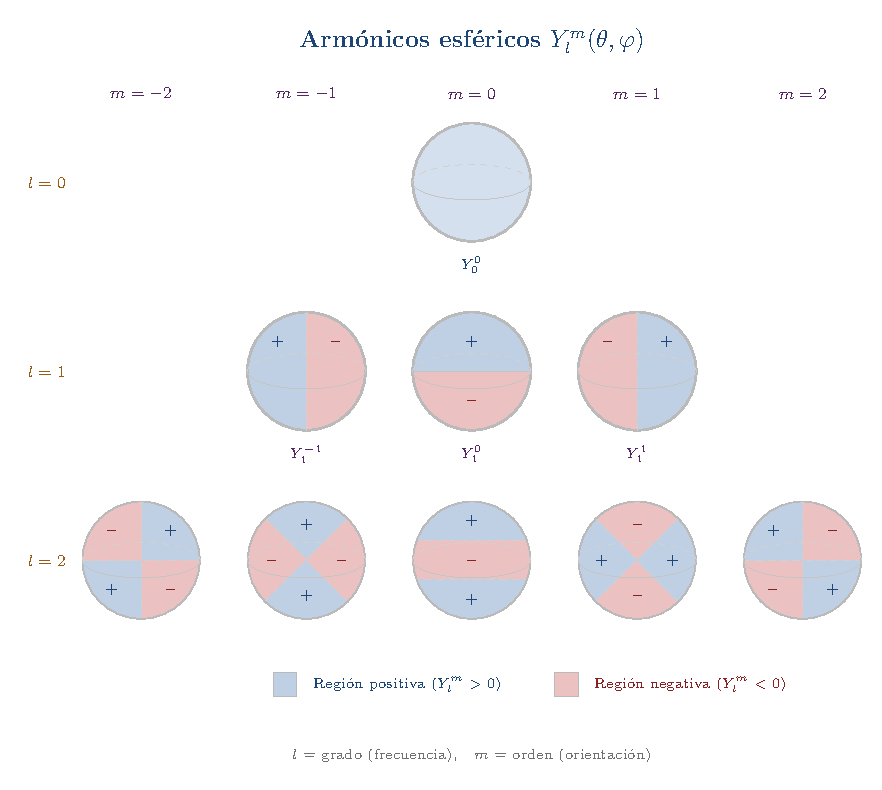
\includegraphics[width=0.85\textwidth]{images/spherical_harmonics.pdf}
    \caption{Spherical harmonics $Y_\ell^m(\theta, \varphi)$ for degrees $\ell = 0, 1, 2$. The blue and red regions indicate positive and negative values, respectively. The degree $\ell$ controls the angular frequency (number of sign changes) and the order $m$ determines the orientation of the nodal pattern. These functions form the basis of the irreducible representations of $SO(3)$ of dimension $2\ell+1$ used in the decomposition of equivariant features~\eqref{eq:irrep_decomposition}.}
    \label{fig:spherical_harmonics_attention}
\end{figure}

In the context of equivariant attention mechanisms, the features in each layer decompose according to representation types:

\begin{equation}
    \mathbf{f} = \bigoplus_{\ell=0}^{L_{\max}} \mathbf{f}^{(\ell)}, \quad \mathbf{f}^{(\ell)} \in \mathbb{R}^{n_\ell \times (2\ell+1)}
    \label{eq:irrep_decomposition}
\end{equation}

where $\mathbf{f}^{(\ell)}$ contains $n_\ell$ channels of type $\ell$, each transforming as a spherical harmonic of degree $\ell$ under rotations.

\paragraph{Clebsch-Gordan Coefficients and Tensor Products}

The composition of features of different types requires the tensor product of irreducible representations. The Clebsch-Gordan coefficients describe how this product decomposes.

\begin{theorem}[Tensor Product Decomposition]\label{thm:tensor_product_so3}
The tensor product of two irreducible representations of $SO(3)$ of degrees $\ell_1$ and $\ell_2$ decomposes as:
\begin{equation}
D^{(\ell_1)} \otimes D^{(\ell_2)} = \bigoplus_{\ell=|\ell_1-\ell_2|}^{\ell_1+\ell_2} D^{(\ell)}
\label{eq:tensor_product_decomposition_attention}
\end{equation}
This decomposition is fundamental for constructing equivariant operations that combine features of different types. The proof is obtained by applying the rule of addition of angular momenta, see \citep{brocker1985representations}.
\end{theorem}

\begin{definition}[Clebsch-Gordan Coefficients]\label{def:clebsch_gordan_attention}
The \textit{Clebsch-Gordan coefficients} $C_{l_1 m_1, l_2 m_2}^{l m}$ (see notation in the file \texttt{notation.tex}) provide the expansion coefficients of the product of spherical harmonics:
\begin{equation}
Y_{\ell_1}^{m_1} \otimes Y_{\ell_2}^{m_2} = \sum_{\ell=|\ell_1-\ell_2|}^{\ell_1+\ell_2} \sum_{m=-\ell}^{\ell} C_{l_1 m_1, l_2 m_2}^{l m} Y_{\ell}^{m}
\label{eq:clebsch_gordan_expansion}
\end{equation}
These coefficients satisfy orthogonality relations and can be computed via recursive formulas or precomputed tables.
\end{definition}

\begin{example}[Low-Degree Cases]\label{ex:low_degree_clebsch_gordan}
To illustrate concretely, consider some low-degree cases:

\textbf{Product $\ell_1 = 0, \ell_2 = 1$} (scalar $\times$ vector):
\begin{equation}
D^{(0)} \otimes D^{(1)} = D^{(1)}
\end{equation}
This product preserves the vector type, simply scaling the vector.

\textbf{Product $\ell_1 = 1, \ell_2 = 1$} (vector $\times$ vector):
\begin{equation}
D^{(1)} \otimes D^{(1)} = D^{(0)} \oplus D^{(1)} \oplus D^{(2)}
\end{equation}
This product generates a scalar ($\ell=0$, the dot product), a pseudovector ($\ell=1$, the cross product), and a symmetric traceless tensor ($\ell=2$).
\end{example}

\textbf{Application in Equivariant Attention.} In equivariant attention mechanisms such as SE(3)-Transformers \citep{fuchs2020se3transformers} and Equiformer \citep{liao2022equiformer}, the tensor products via Clebsch-Gordan coefficients allow:
\begin{itemize}
    \item \textbf{Combining queries and keys}: $\mathbf{q}_i^{(\ell_1)} \otimes \mathbf{k}_j^{(\ell_2)}$ to compute equivariant attention scores
    \item \textbf{Mixing geometric information}: Incorporating relative directions $\hat{\mathbf{r}}_{ij}$ (type $\ell=1$) with node features
    \item \textbf{Maintaining exact equivariance}: Each operation respects the group structure of $SO(3)$ by construction
\end{itemize}

\begin{example}[Feature Space Decomposition]\label{ex:feature_space_decomposition}
Consider a feature space with $L_{\max} = 2$:
\begin{align}
\mathbf{f} &= \mathbf{f}^{(0)} \oplus \mathbf{f}^{(1)} \oplus \mathbf{f}^{(2)} \\
&= \underbrace{\mathbb{R}^{n_0 \times 1}}_{\text{scalars}} \oplus \underbrace{\mathbb{R}^{n_1 \times 3}}_{\text{vectors}} \oplus \underbrace{\mathbb{R}^{n_2 \times 5}}_{\text{degree-2 tensors}}
\label{eq:feature_space_example}
\end{align}

An equivariant attention operation computes:
\begin{equation}
e_{ij} = \sum_{\ell_q, \ell_k, \ell_{\text{out}}} \text{MLP}_{\ell_q, \ell_k, \ell_{\text{out}}} \left( \mathbf{q}_i^{(\ell_q)} \otimes \mathbf{k}_j^{(\ell_k)} \right)^{(\ell_{\text{out}})}
\label{eq:equivariant_attention_score_irreps}
\end{equation}

where the tensor product decomposes according to Equation~\eqref{eq:tensor_product_decomposition_attention} and the MLPs operate independently on each representation type.
\end{example}

\subsection{Equivariant Architectures}\label{sec:equivariant_transformers}

\subsubsection[SE(3)-Transformers]{SE(3)-\glspl{Transformer}}

The SE(3)-\glspl{Transformer} of \citet{fuchs2020se3transformers} extend attention to be equivariant under rotations and translations in 3D.

For scalar features $f_0$, vector features $\mathbf{f}_1$, and higher-order tensor features, the attention is constructed as:

\begin{align}
    f_0^{\text{out}} &= \sum_j \alpha_{ij} f_{0,j} \\
    \mathbf{f}_1^{\text{out}} &= \sum_j \alpha_{ij} \mathbf{f}_{1,j} \\
    \alpha_{ij} &= \text{softmax}(\text{\gls{MLP}}(f_{0,i}, f_{0,j}, \|\mathbf{r}_{ij}\|, \mathbf{f}_{1,i} \cdot \mathbf{f}_{1,j}))
    \label{eq:se3_transformer_attention}
\end{align}

where $\mathbf{r}_{ij} = \mathbf{r}_i - \mathbf{r}_j$ is the relative position vector.

\begin{theorem}[SE(3)-Equivariance of Attention]
    The attention mechanism defined in equation~\eqref{eq:se3_transformer_attention} is equivariant under the group $SE(3)$ of Euclidean rotations and translations \citep{fuchs2020se3transformers}.
\end{theorem}

\begin{proof}
Let $(R, \mathbf{t}) \in SE(3)$ be a roto-translation. The attention weights $\alpha_{ij}$ depend on: (i) scalars $f_{0,i}, f_{0,j}$ (invariant by definition), (ii) the norm $\|\mathbf{r}_{ij}\| = \|\mathbf{r}_i - \mathbf{r}_j\|$ which is invariant under $SE(3)$: $\|R\mathbf{r}_i + \mathbf{t} - R\mathbf{r}_j - \mathbf{t}\| = \|R(\mathbf{r}_i - \mathbf{r}_j)\| = \|\mathbf{r}_i - \mathbf{r}_j\|$, and (iii) $\mathbf{f}_{1,i} \cdot \mathbf{f}_{1,j}$ which is invariant since $\mathbf{f}_1$ transforms as a type-1 vector under $SO(3)$: $(R\mathbf{f}_{1,i}) \cdot (R\mathbf{f}_{1,j}) = \mathbf{f}_{1,i} \cdot \mathbf{f}_{1,j}$. Therefore, the scores $\alpha_{ij}$ are \emph{invariant} under $SE(3)$.

For the vector output: $\mathbf{f}_1^{\text{out}} = \sum_j \alpha_{ij} \mathbf{f}_{1,j}$. Under $(R, \mathbf{t})$: $\sum_j \alpha_{ij} R\mathbf{f}_{1,j} = R \sum_j \alpha_{ij} \mathbf{f}_{1,j} = R \mathbf{f}_1^{\text{out}}$. Thus, the type-1 output is \emph{equivariant}. The scalar (type-0) outputs are trivially invariant.
\end{proof}

\subsubsection{Equiformer: Equivariant \gls{MLP} Attention}

The Equiformer of \citet{liao2022equiformer} surpasses the traditional dot product through equivariant \gls{MLP}-based attention.

Instead of the dot product $\mathbf{q}_i^T \mathbf{k}_j$, it uses:

\begin{equation}
    e_{ij} = \text{\gls{MLP}}_{\text{attn}}(\mathbf{q}_i \otimes \mathbf{k}_j, \|\mathbf{r}_{ij}\|)
    \label{eq:equiformer_attention_scores}
\end{equation}

where $\otimes$ denotes the tensor product of irreducible features.

The tensor product of irreducible representations decomposes as:

\begin{equation}
    D^{(\ell_1)} \otimes D^{(\ell_2)} = \bigoplus_{\ell=|\ell_1-\ell_2|}^{\ell_1+\ell_2} D^{(\ell)}
    \label{eq:tensor_product_decomposition}
\end{equation}

This construction preserves SO(3) equivariance while allowing richer interactions than the simple dot product.

\subsubsection{Lie\gls{Transformer}: General Framework}

The Lie\gls{Transformer} of \citet{hutchinson2020lietransformer} provides a unified framework for attention equivariant to arbitrary Lie groups.

The approach is based on ``lifting'' the representations to the group:

\begin{enumerate}
    \item \textbf{Lift}: $\mathbf{x} \mapsto \{(g, \mathbf{x})\}_{g \in G}$
    \item \textbf{Process}: Apply attention in the group space
    \item \textbf{Project}: Reduce back to the original space
\end{enumerate}

\begin{equation}
    \text{LieAttn}(\mathbf{x}) = \text{Project}(\text{Attention}(\text{Lift}(\mathbf{x})))
    \label{eq:lie_attention}
\end{equation}

For a group $G$, the left regular representation is defined as:

\begin{equation}
    (L_g f)(h) = f(g^{-1}h), \quad g, h \in G, f \in L^2(G)
    \label{eq:left_regular_representation}
\end{equation}

This construction guarantees equivariance for any Lie group.

\subsubsection{EPT: Equivariant Foundation Models}

The Equivariant Pretrained Transformer (EPT) of \citet{jiao2024ept} represents the first foundation model that unifies the geometric learning of small molecules and proteins under an equivariant framework.

\begin{definition}[Multi-Domain Equivariant Pretraining]
    A foundation model $F_{\text{EPT}}$ is multi-domain equivariant if for domains $\mathcal{D}_1, \mathcal{D}_2$ (e.g., molecules, proteins) and group $G$:
    \begin{equation}
        F_{\text{EPT}}(g \cdot \mathbf{x}) = g \cdot F_{\text{EPT}}(\mathbf{x}), \quad \forall \mathbf{x} \in \mathcal{D}_1 \cup \mathcal{D}_2, g \in G
        \label{eq:multi_domain_equivariance}
    \end{equation}
\end{definition}

The EPT architecture incorporates enhanced representation blocks:

\begin{equation}
    \mathbf{h}_i^{\text{EPT}} = \text{E(3)-TransformerBlock}(\mathbf{h}_i, \{\mathbf{h}_j\}_{j \in \mathcal{N}_{\text{ext}}(i)})
    \label{eq:ept_enhanced_block}
\end{equation}

EPT uses multiple pretraining objectives that preserve geometry:

\begin{align}
    \mathcal{L}_{\text{EPT}} &= \mathcal{L}_{\text{masked}} + \mathcal{L}_{\text{geom}} + \mathcal{L}_{\text{cross}} \\
    \mathcal{L}_{\text{geom}} &= \|\mathbf{f}(g \cdot \mathbf{x}) - g \cdot \mathbf{f}(\mathbf{x})\|^2 \\
    \mathcal{L}_{\text{cross}} &= \text{KL}(\mathbf{p}_{\text{mol}}, \mathbf{p}_{\text{prot}})
    \label{eq:ept_loss}
\end{align}

\begin{proposition}[Transfer of Geometric Knowledge]
    If a model $F$ is pretrained on a domain $\mathcal{D}_1$ with $G$-equivariance, then the transfer to a domain $\mathcal{D}_2$ with the same symmetry $G$ preserves the equivariance properties \citep{jiao2024ept}.
\end{proposition}

\begin{proof}
If $F$ is $G$-equivariant, this means its layers are built with equivariant operations (tensor products, group convolutions, equivariant linear layers). Equivariance is an \emph{architectural} property; it does not depend on the training data nor on the values of the learned parameters. When transferring $F$ to $\mathcal{D}_2$ (with or without fine-tuning), the structure of the layers does not change, so $F(g \cdot \mathbf{x}) = g \cdot F(\mathbf{x})$ holds for all $g \in G$ and $\mathbf{x} \in \mathcal{D}_2$. The necessary condition is that both domains admit the same action of the group $G$.
\end{proof}

\subsection{Equivariant Attention on Point Clouds}

3D point clouds present unique challenges for attention due to their unstructured nature and the need to preserve equivariance under rigid transformations.

\subsubsection{Point \gls{Transformer}: Vector Attention}

The Point \gls{Transformer} of \citet{zhao2021point} introduces vector attention specifically designed for point clouds:

\begin{equation}
    \mathbf{y}_i = \sum_{j \in \mathcal{N}(i)} \rho(\gamma(\phi(\mathbf{x}_i) - \psi(\mathbf{x}_j) + \delta))(\alpha(\mathbf{x}_j) + \delta)
    \label{eq:point_transformer_attention}
\end{equation}

where:
\begin{itemize}
    \item $\phi, \psi, \alpha$ are linear transformations
    \item $\delta = \text{\gls{MLP}}(\mathbf{p}_i - \mathbf{p}_j)$ encodes positional information
    \item $\gamma, \rho$ are \glspl{MLP}
\end{itemize}

The function $\delta$ captures the local geometry:

\begin{equation}
    \delta_{ij} = \text{\gls{MLP}}(\mathbf{p}_i - \mathbf{p}_j, \|\mathbf{p}_i - \mathbf{p}_j\|)
    \label{eq:positional_encoding_3d}
\end{equation}

The Point \gls{Transformer} formulation can be understood as an instance of the equivariant attention framework developed in \autoref{subsec:equivariant_attention}. The positional encoding $\delta_{ij}$ depends exclusively on the relative position $\mathbf{p}_i - \mathbf{p}_j$, which is invariant under translations. Likewise, if the \gls{MLP} that computes $\delta$ receives as input only the relative difference and its norm, the architecture is invariant under rotations in the computation of the attention weights, connecting directly with the invariance condition of the compatibility functions of \autoref{subsec:equivariant_attention}. Vector attention (in contrast to standard scalar attention) allows different dimensions of the attention vector to independently modulate the features, providing greater expressive capacity than a single scalar weight $\alpha_{ij}$ per pair of points.

A computational advantage of the Point \gls{Transformer} over architectures such as SE(3)-\glspl{Transformer} lies in avoiding the tensor product of irreducible representations (Equation~\eqref{eq:tensor_product_decomposition_attention}), which has cost $O(\ell_{\max}^3)$ for maximum degree $\ell_{\max}$. By operating directly on differences of positions and features, the Point \gls{Transformer} achieves complexity $O(|\mathcal{N}(i)| \cdot d)$ per point, at the cost of giving up exact equivariance under $SO(3)$ for the output features (only the relative positions are invariant, not the transformed features).
